\documentclass[11pt, a4paper, oneside, openright]{article} %draft

%Document settings

%\setlength{\parindent}{0cm}


%Packages
\usepackage{graphicx,color}
\usepackage{amssymb, amsmath, array}

\usepackage[english]{babel}
\usepackage[utf8]{inputenc}
\usepackage{parskip}

\usepackage[nottoc]{tocbibind}
\usepackage{cite}

\usepackage{tikz}
\usetikzlibrary{shapes.geometric}

\usepackage{listings}
\usepackage{listings-golang}

\lstset{ % add your own preferences
   frame=single,
    basicstyle=\footnotesize,
    keywordstyle=\bf{\color{red}},
    numbers=left,
    numbersep=5pt,
    showstringspaces=false, 
    stringstyle=\color{olive},
    tabsize=4,
    language=Golang % this is it !
}

\usepackage{enumitem}
\setlist{noitemsep}
\setlist[enumerate]{itemsep=0.2em,topsep=0pt,parsep=0pt,partopsep=0pt}
\setlist[itemize]{itemsep=0.2em,topsep=0pt,parsep=0pt,partopsep=0pt}

\usepackage{hyperref}

\begin{document}

\input{cover}
\pagebreak
\pagestyle{empty}
\listoffigures

\pagebreak
\tableofcontents

\pagebreak

\pagestyle{plain}
\section{Introduction}
\setcounter{page}{1}

Nowadays, real-time collaborative editing tools are well-known and almost daily used amongst students and employees who need an easy and ready-to-use solution to work on a common project. In contrast to version control systems like Git, users must be able to edit the same document simultaneously and at any time. The changes inferred by one user need to be integrated at every other site and the algorithm must converge towards a unique definitive document version. The most popular and used amongst current implementations are Etherpad and Google Docs, the latter having been launched in 2007.

Despite their accessibility and convenience of use, those existing systems rely on a central organ to process and redistribute operations generated at each site. This involves the loss of control over the data by users. In other words, current solutions infer a trust relation between users and the service provider. Possible system failure or data leakage towards other organizations might break this trust relation. 

This problem can be addressed by using a distributed and independent algorithm, which communicates by secured peer-to-peer communication between sites. Collaborative groups can now have ultimate control over their data, communication and how different sites converge to a definitive version of their document.

The task is to implement an admissibility based operational transformation algorithm for peer-to-peer collaborative editing (ABTU) and evaluate its performance.
The algorithm will be based on \cite{abtu} and \cite{abtuu}. This algorithm is the only one that has been proved to enable parties to converge their state in a peer-to-peer configuration. The possibility to undo any changes is also a key feature of such an algorithm and must therefore also be implemented. This part will be based on [reference.] The programming language of choice for the backend in this project will be Go!.

In order to complete this task, one will first have to study the ABTU algorithm. In parallel, the implementation of peer-to-peer communication will be done to learn the programming language. After having finished the implementation of the algorithm, testing will take place. The last part will be to define limitations and further improvement to be done.

Firstly, goals for the project will be further defined. The paper will then go through an introduction on operational transformation and the algorithm which will be used. The design and implementation will be precisely explained. Results and limitations of the project will be presented and lead to a discussion on the improvements and future work to be done. Details about the installation will be provided in the appendix.


%-------------------------------------------------------------------------------------------------------
\section{Goals}
\label{sec:motiv}

In this section, we will further define the goals of this project. 

The algorithm which will be implemented is part of a software which is organized as follows. The graphical interface and database management are implemented in JavaScript, this represents the frontend. The ABTU algorithm is implemented in Go. The two parts are linked by a management part, also implemented in Go, which handles different instances of the ABTU algorithm and the communication with other peers. The ABTU algorithm and the management represent the backend.

The goals for this project are:

\begin{enumerate}
	\item Implement peer-to-peer communication between to sites.
	\item Design and implement the ABTU algorithm and the interface with the management.
\end{enumerate}


If the two first goals are achieved and time is left, the next goals are:

\begin{enumerate}
	\setcounter{enumi}{2}
	\item Test the implementation of the ABTU algorithm.
	\item Evaluate the performance of the ABTU algorithm.
	\item Link the implementation of the ABTU algorithm with the management and the frontend.

\end{enumerate}

%-------------------------------------------------------------------------------------------------------
\section{Corresponding Background}
\label{sec:background}

%----------------------------------------------------------------------
\subsection{Operational Transformation}
\label{subsec:optransform}

The ABTU algorithm is based on operational transformation, this subsection will introduce this concept.

A document is represented by a string of characters. The positions of the characters start from 0 and increase until the end of the document. A modification of the document is represented by two types of operations: insertions (INS) and deletions (DEL). As we will see, the identity of the site at which the operation was generated is also important. An operation is therefore defined by its site identity, type, position and character: $OP(siteId, type, position, character)$.

In figure~\ref{fig:simpleOp}, the initial state of the document is "abc". We apply the operation $OP(1, INS, 4, d)$, and the resulting string is "abcd".

\begin{figure}[h]
\begin{center}
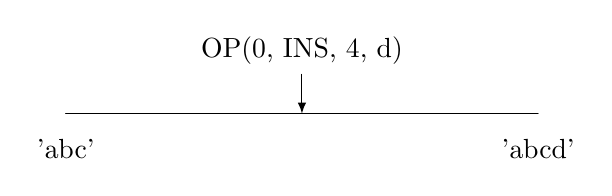
\begin{tikzpicture}[scale=1,cap=round]
\draw (-3, 0) -- (3, 0);

\draw (-3, -0.2) node[below] {'abc'};
\draw (3, -0.2) node[below] {'abcd'};

\draw [-latex] (0, 0.5) -- (0, 0);
\draw (0, 0.5) node[above] {OP(0, INS, 4, d)};


\end{tikzpicture}
\end{center}
\caption{Execution of an Operation on a String. Own Illustration\label{fig:simpleOp}}
\end{figure}

In collaborative editing, multiple users simultaneously generate operations at different site, this means that they edit the document concurrently. When an operation is generated at one site, it is first applied to the local copy of the document and then distributed to other peers. Therefore, at a given time, two sites do not necessarily have the same version of the document.

The following example from figure~\ref{fig:concurrentOp}  will show why operations need to be transformed. Starting from the same document state "abc", site $1$ and $2$ respectively generate, apply and distribute operations $o_1 = OP(1, INS, 0, z)$ and $o_2= OP(2, DEL, 3, c)$. After site $1$ has executed operation $o_1$, its state is "zabc", one easily see that the operation $o_2$ no longer has the desired effect on the document: instead of deleting the character "c", it would remove "b", resulting in the state "zac". This example illustrates the fact that operation $o_2$ should be transformed to $o_2 = OP(2, DEL, 4, z)$. On the contrary, at site $2$, the operation $o_2$ is already valid in the document state ‘ab’. This is what is called \textit{operational transformation}.


\begin{figure}[h]
\begin{center}
\begin{tikzpicture}[scale=1,cap=round]
\draw (-5, 3.5) node[above] {Site $1$};
\draw (-5, 3) -- (-5, -3);

\draw (-5.2, 3) node[left] {"abc2};
\draw (-4.8, 1.5) node[right] {$o_1 = OP(1, INS, 0, z')$};
\draw (-5.2, 0) node[left] {"zabc"};
\draw (-4.8, -1.5) node[right] {$o_2$};
\draw (-5.2, -3) node[left] {"zac"};


\draw (5, 3.5) node[above] {Site $2$};
\draw (5, 3) -- (5, -3);

\draw (5.2, 3) node[right] {"abc"};
\draw (4.8, 1.5) node[left] {$o_2 = OP(2, DEL, 4, c)$};
\draw (5.2, 0) node[right] {"ab"};
\draw (4.8, -1.5) node[left] {$o_1$};
\draw (5.2, -3) node[right] {"zab"};

%arrows
\draw [-latex] (-4.8, 1.3) -- (4.8, -1.3);
\draw [-latex] (4.8, 1.3) -- (-4.8, -1.3);


\end{tikzpicture}
\end{center}
\caption{Generation of two Concurrent Operations. Own Illustration.\label{fig:concurrentOp}}
\end{figure}

When multiple collaborators are editing a document concurrently, operations must be verified and transformed if necessary before being applied to the local copy of the document, this is what the ABTU algorithm handles.

%----------------------------------------------------------------------
\subsection{ABTU Algorithm}
\label{subsec:abtu}

In this subsection, notions about the framework of the algorithm and notations from \cite{abtu} and \cite{abtuu} will first be introduced, the algorithm will then be described.

%--------------------------------------------
\subsubsection{Notions and Notations}

\textbf{Operation} As seen in section~\ref{subsec:optransform}, an operation is defined by its site id: $o.id$, type: $o.t$, character: $o.c$ and position: $o.p$.

\textbf{Definition state:} The definition state $dst(o)$ of an operation $o$, is the state of the document in which the operation has been generated. The result of the execution of $o$ in $dst(o)$ is written $dst(o) \circ o$.

We note $o_1 \sqcup o_2$ if both operation $o_1$ and $o_2$ have the same definition state $dst(o_1) = dst(o_2)$ and $o_1 \mapsto o_2$ if $dst(o_1) \circ o_1 = dst(o_2)$.

\textbf{Operation sequence:} The execution of a sequence of operations $sq = [o_1, o_2, \cdots, o_n]$ is the result of the consecutive execution of its operations to the definition state of $o_1$: $dst(o_1) \circ o_1 \circ o_2 \circ \cdots \circ o_n = dst(o_1) \circ sq $. Two operation sequences $sq_1$ and $sq_2$ are equivalent if $ dst(sq_1) = dst(sq_2)$ and $dst(sq_1) \circ sq_1 = dst(sq_2) \circ sq_2$.

\textbf{Vector time and timestamp:} In order to keep track of time in multiple places, the ABTU algorithm uses the concept of vector clock. For $n$ sites, the time is represented by an array of integers of length $n$. Time increases as operations are applied at each site.

Each site has its own time vector $SV$. When an operation is generated at site $i$, the time vector $SV_i$ is incremented by $1$ at index $i$: $SV_i[i] = SV_i[i] + 1$. When a remote operation from site $j$ is integrated at site $i$, $SV_i$ is incremented at index $j$.

Time vectors can be partially ordered: $t_1 < t_2$ iff $\forall _i: t_1[i] \leq t_2[i]$ and  $\exists _j : t_1[j] < t_2[j]$.

An operation also carries its own timestamp $o.v$. For an operation $o$ generated at site $i$, $o.v$ is the time $SV_i$ from site $i$ at which $o$ was generated. We write $o_1 \rightarrow o_2$ if $o_1.v < o_2.v$ and we say that $o_1$ and $o_2$ are concurrent ($o_1\ || \ o_2$) if neither $o_1 \rightarrow o_2$ nor $o_2 \rightarrow o_1$ hold.

\textbf{Effects relation:} A first definition can be given as follows: $a \prec b$ if the position of $a$ is smaller than the position of $b$ in the document.

However, this definition is not entirely satisfactory, this can be shown by an example from \cite{abtuu} in figure~\ref{fig:effectrel}. Three sites start with the same state "ab", the effect relation is a $\prec$ b. Site $2$ first generates $OP(2, INS, x, 2)$ and then receives $OP(1, DEL, 0, a)$ and $OP(1, DEL, 0, b)$ from site $1$ and then $OP(3, INS, x, 1)$ from site $3$.

As x and y were not generated at the same site, there is no direct effect relation between them, but it is still possible to order them by transitivity. As a $\prec$ b $\prec$ x and y $\prec$ a $\prec$ b, by transitivity y $\prec$ a $\prec$ b $\prec$ x and y $\prec$ x.

If two sites concurrently insert a character at the same position, the ordering is made accordingly to the id of both sites.

\begin{figure}[h]
\begin{center}
\begin{tikzpicture}[scale=1,cap=round]


\draw (0, 1.5) -- (0, -1.5);
\draw (0, 2.5) node[above] {Site $0$};
\draw (0, 2) node[above] {'ab'};

\draw (-0.2, 1.5) node[left] {$OP(2, INS, 0, x)$};
\draw (-2, 0.5) node[left] {$OP(1, DEL, 0, a)$};
\draw [-latex] (-2, 0.5) -- (-0.2, 0.5);

\draw (-2, -0.5) node[left] {$OP(1, DEL, 0, a)$};
\draw  [-latex](-2,  -0.5) -- (-0.2, -0.5);

\draw (2, -1.5) node[right] {$OP(3, INS, 0, y)$};
\draw  [-latex] (2, -1.5) -- (0.2, -1.5);

\end{tikzpicture}
\end{center}
\caption{Effects Relation. Own Illustration.\label{fig:effectrel}}
\end{figure}

\textbf{Effects relation order:} A sequence of operation is said to be in effects relation order if its operations are ordered according to the effect relation of their characters. This order is denoted by $<_e$,  $=_e$ and $>_e$.

For two operations $o_1$ and $o_2$ where $o_1 \sqcup o_2$ holds, $o_1 <_e o_2$ if (1) $o_1.p < o2.p$; (2) $ o_1.p = o_2.p, o_1.t = INS, o_2.t = DEL$ ; or (3) $o_1.p = o_2.p, o1.t = o_2.t = INS, o_1.id < o_2.id$. When $o_1 \mapsto o_2$ holds, $o_1 <_e o_2$ if (1) $o_1.p < o2.p$; (2) $o_1.p = o_2.p, o1.t = o_2.t = DEL$.

The $>_e$ operator is completely symmetric to $<_e$, and $o_1 =_e o_2$ is true if neither $<_e$ nor $>_e$ hold.

%--------------------------------------------
\subsubsection{Undo of Operations}

The undoing of an operation can simply be achieved by generating and executing its inverse operation. However, there are some subtleties to this process.

If $o$ is an undo operation, $o.ov$ is the timestamp of the operation it undoes.

As an operation cannot be undone twice, we use $o.uv$ as the set of timestamps of operations that undo (or try to re-undo) $o$. When an operation is undone twice, the two undo operation get merged into one. Their respective timestamps also get merged to form sets of timestamps.

Some operations cannot be undone. If we have $o_1 = OP(1, INS, 0, a)$ and $o_2 = OP(1, DEL, 0, a)$ then $o_1$ can no longer be undone because $o_2$ is dependent on $o_1$. To keep track of those dependencies, $o.dv$, the set of timestamps of operations that depend on $o$ is used.

The set of timestamps $o.tv$ contains the timestamps of all operations whose effect objects are identical to $o.c$.

%--------------------------------------------
\subsubsection{Description of the Algorithm}

The ABTU algorithm is based on two important principles which are \textit{Causality Preservation} and \textit{Admissibility Preservation}.

\textbf{Causality Preservation:} Causality is preserved if, for any two operations $o_1$ and $o_2$, if $o_1 \rightarrow o_2$, then $o_1$ must be invoked before $o_2$ at any site. Therefore, a remote operation from site $j$ is \textit{causally ready} at site $i$ iff $\forall_{k\neq j} SV_i[k] \leq o.v[k]$ and $o.v[j] = SV_i[j] + 1$. If remote operations are only executed when they are causally ready, causality preservation is respected.

\textbf{Admissibility Preservation: } Admissibility is preserved if the execution of any operation respects the effects relation $\prec$ of the system. At any site, remote operation must be transformed so that they become admissible and can be executed.

As seen in~\ref{subsec:optransform}, before being executed, remote operations need to be transformed. In order to transform operations against each other, each site must maintain a history buffer $H$ of every operation already executed. $H$ is an operation sequence maintained in effects relation order. When remote operations are received, each site will transform, execute and integrate them into $H$.

When an undo operation is generated, the original operation must be recovered from the history buffer and its inverse generated. The undo operation is then executed, distributed and stored just after the original operation in $H$.

The ABTU algorithm has been proved to converge at some point in the future, i.e. all history buffers in all sites of the system will, at some point, end up to be equivalent sequences of operations.

Both local and remote operations need to be handled by the ABTU algorithm. The psoeudocode for the described functions is available in Appendix~\ref{appa}.

\textbf{Local Operations}

 Local operation must be timestamped, integrated into $H$ and distributed to other peers, this is done by \textit{localThread} and \textit{integrateL} functions.

\textbf{Function localThread:} When an operation $o$ is generated at site $i$, function localThread simply increments $SV_i[i]$, adds this timestamp to $o$, calls integrateL and propagates the result to other sites.

If the operation is an undo, localThread searches the original operation $o$ in $H$, and checks if an undo is possible with $o.uv$ and $o.dv$. It then generates its inverse and sets all the necessary timestamps. The time $SV_i[i]$ is then incremented, integrateL called and the result distributed.

\textbf{Function integrateL:} Function integrateL scans $H$ from right to left and modifies the position of all operations $H[k]$ as long as $H[k] <_e o$. If $H[k] =_e o$, $o.tv$ and $H[k].dv$ are set accordingly. It is important to notice that $H[j] \mapsto o$ to make the correct checks for the $<_e$ relation. 

For an undo operation $u$, the index $j$ in $H$ of the original operation is recovered with the help of $u.uv$. All operations $H[k] \ \forall_{k>j}$ are transformed against $u$ and $u$ is inserted at position $k+1$.

\textbf{Remote Operations}

Remote operations are first stored in a receiving buffer $RB$. When no local operation has to be integrated, the \textit{remoteThread} and \textit{integrateR} function can transform, integrate and execute the first causally ready operation from $RB$.

\textbf{Function remoteThread:} When a causally ready operation form site $j$ is integrated at site $i$, the remoteThread function calls integrateR and increments $SV_i[j]$.

If the operation is an undo $u$, the original operation $o$ is also recovered from $H$ and $o.uv$ is set to $u.v$. If $o.uv \neq \empty$, then $o$ has already been undone by some operation $u'$. The timestamps of $u'$ are updated accordingly and $u$ discarded.
The time $SV_i[j]$ is then incremented, integrateR called and the result distributed.


\textbf{Function integrateR:} The function integrateR serves two purposes: 

\begin{enumerate}
	\item Transform $o$ against all operations $H[k]$ where $o\ ||\ H[k]$ holds and integrate $o$ in $H$. Indeed, at the generation of $o$, $H[k]$ was unknown to the site $j$ and therefore $o$ has not taken into account $H[k]$. As $H$ is sorted in effects relation order, the transformation must only be done as long as $H[k] <_e o$. It is important to notice that $H[k] \sqcup o$ holds when the $<_e$ check is made.
	\item Transform all operations $H[k]$ for which $H[k] >_e o$ is true against $o$.
\end{enumerate}

If the operation is an undo $u$, the original operation $o$ is recovered from $H$ with the help of $o.tv$ and $u.p$ is set to $o.p + 1$. $H$ is then scanned from left to right, starting from $o$, to integrate the effect of concurrent operation whose effect object are identical to $u.c$. If $\exists H[k]$ s.t. $H[k] =_e u$, then $o$ has already been undone by $H[k]$ and the two operations are merged. The operation $u$ is finally integrated into $H$ just after $o$ and executed.


%-------------------------------------------------------------------------------------------------------
\section{Design and Implementation}
\label{sec:designimplementation}

As explained in section \ref{sec:motiv}, the general structure of the software is organized in three parts. The frontend manages the interaction with the user and the database. It is coded in JavaScript.
The ABTU algorithm is implemented in Go and represented by an $ABTUInstance$ structure. Communication with the ABTU instance is made through four different channels.
The management, also implemented in Go, manages different instances of the ABTU algorithm, handles the communication between frontend and the ABTU instance, and the communication with other peers.
The communication between frontend and backend is done through a web socket.

The design of the model has been modularized to allow for greater flexibility: the ABTU instance can be simply be plugged in any management and frontend which respect the interface and the communication protocol.

\begin{figure}[!h]
\begin{center}
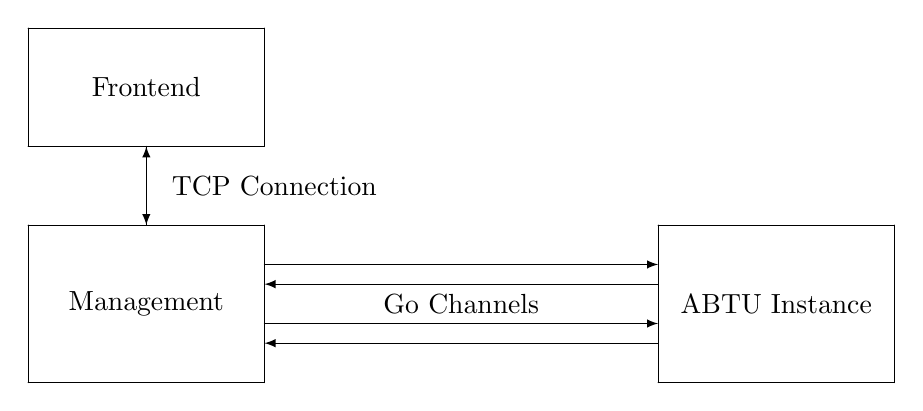
\begin{tikzpicture}[scale=1,cap=round, square/.style={regular polygon,regular polygon sides=4}]

\node at (-4.5, 1.75) {Frontend};
\draw (-6, 2.5) -- (-6, 1);
\draw (-6, 1) -- (-3, 1);
\draw (-3, 1) -- (-3, 2.5);
\draw (-3, 2.5) -- (-6, 2.5);

\node at (-4.5, -1) {Management};
\draw (-6, -0) -- (-6, -2);
\draw (-6, -2) -- (-3, -2);
\draw (-3, -2) -- (-3, -0);
\draw (-3, -0) -- (-6, -0);

\node at (3.5, -1) {ABTU Instance};
\draw (2, -0) -- (2, -2);
\draw (2, -2) -- (5, -2);
\draw (5, -2) -- (5, -0);
\draw (5, -0) -- (2, -0);

\node at (-4.3, 0.5) [right] {TCP Connection};
\draw [-latex] (-4.5, 1) -- (-4.5, 0);
\draw [-latex] (-4.5, 0) -- (-4.5, 1);

\node at (-0.5, -1) {Go Channels};
\draw [-latex] (-3, -0.5) -- (2, -0.5);
\draw [-latex] (2, -0.75) -- (-3, -0.75);
\draw [-latex] (-3, -1.25) -- (2, -1.25);
\draw [-latex] (2, -1.5) -- (-3, -1.5);
\end{tikzpicture}
\end{center}
\caption{General Organization of the Software. Own Illustration.\label{fig:softgen}}
\end{figure}

%---------------------------------------------------
\subsection{ABTU Instance}

The ABTUInstance struct is shown in figure~\ref{code:ABTUInstance}. It stores the siteId, site timestamp and history buffer, and uses four channels for the communication with the management.

\begin{figure}[!h]
\begin{center}
\begin{lstlisting}
type ABTUInstance struct {
	id SiteId
	sv Timestamp // Site timestamp
	h []Operation // History buffer
	
	// ...

	// channel for receiving from local frontend
	localToABTU chan []byte 
	// channel for sending to local frontend
	aBTUToLocal chan []byte

	// channel for receiving remote operations
	remoteToABTU chan []byte 
	// channel for dispatching local operations to remote sites.
	aBTUToRemote chan []byte

}
\end{lstlisting}
\end{center}
\caption{ABTUInstance Struct. Own Code.\label{code:ABTUInstance}}
\end{figure}

%---------------------------------------------------
\subsection{Receiving Buffer Manager}

When remote operations are received through the remoteToABTU channel, they must be stored in a receiving buffer. Concurrently, the remote thread reads in the remote buffer to find the first causally ready operation to integrate. There  is a clear need for a concurrent data structure in this situation,  the \textit{receivingBufferManager} (rbm) serves this purpose. This data structure is inspired from \cite{datastruct}.

As shown in figure \ref{code:rbm1}, requests to the datastructure are represented by structs, containing a return channel, and sent through channels to the rbm. The possible requests are adding a remote operation to the buffer, getting the first causally ready operation given a $SV$ or delete the last causally ready operation returned from the buffer.

\begin{figure}[!h]
\begin{center}
\begin{lstlisting}
// A request operation
type GetCausallyReadyOp struct {
	CurrentTime Timestamp
	Return      chan Operation
}

type RemoteBufferManager struct {
	// Channels for requests
	Add chan AddOp
	Get chan GetCausallyReadyOp
	RemoveRearrange chan RemoveRearrangeOp

	// The actual receiving buffer.
	rb []Operation

	// ...
}
\end{lstlisting}
\end{center}
\caption{Receiving Buffer Manager Struct. Own Code.\label{code:rbm1}}
\end{figure}

Once started, the rbm continuously checks for incoming requests by using a select control structure on different channels. When the first causally ready operation is requested, it might still not be present in the buffer, in that case, the rbm checks the \textit{aBTUIsWaitingCausallyReadyOp} flag, handles other requests and sends the operation when it is available. Figure~\ref{code:rbm2} shows a simplified version of the control structure.

\begin{figure}[!h]
\begin{center}
\begin{lstlisting}
func (rbm *RemoteBufferManager) Start(rb []Operation){
	// ...

	// Used to manage pending GetCausallyReadyOp requests
	rbm.aBTUIsWaitingCausallyReadyOp = false

	go func () {
		for {
		select {
		case addOp := <- rbm.Add:
			rbm.rb = append(rbm.rb, addOp.Operation)
			addOp.Ack <- true
			// If ABTU is waiting for a causally ready operation
			if rbm.aBTUIsWaitingCausallyReadyOp {
				// Get causally ready op
				// If present:
				// sent it through rbm.causallyReadyOpRetChan
				// set rbm.aBTUIsWaitingCausallyReadyOp = false
			}
		// Return the first causally ready operation if available
		case getCausallyReadyOp := <- rbm.Get:
			// Get causally ready op
			// If present:
			// sent it through rbm.causallyReadyOpRetChan
			// and set rbm.aBTUIsWaitingCausallyReadyOp = false
			//  If not present:
			// set rbm.aBTUIsWaitingCausallyReadyOp = true
		case removeRearrangeOp := <- rbm.RemoveRearrange:
			// remove the last causally ready op from the buffer
		}
	}
}()
}
\end{lstlisting}
\end{center}
\caption{Receiving Buffer Manager Control Structure. Own Code.\label{code:rbm2}}
\end{figure}



%---------------------------------------------------
\subsection{Communication with Frontend}

When the user generates a new operation, it is directly executed on the document in the frontend, and then sent to the ABTU instance for integration and distribution. If the operation is an undo, the frontend sends an undo request to the ABTU instance and waits for the operation. When a remote operation is handled in the ABTU instance, the resulting operation must be sent to the frontend.

Priority is given to local operations on remote ones. When a local operation $o$ is created, $o$ must be integrated into $H$ before any other remote operation. If this is not the case, then the processing of the remote operation will not take into account $o$ and the result will not be valid in the already modified state of the document. This problem can be illustrated by the following set of events. The starting state of the document is 'abc'.

\begin{enumerate}
\item User generates operation $o_l = OP(1, INS, 0,  x)$ and sends it to ABTU.
\item ABTU integrates remote operation $o_r = OP(2, DEL, 3, c)$. The definition state of $o_r$ is "abc". The goal of $o_r$ is to remove "c" from the document.
\item ABTU sends the resulting operation $o_r$, which remains unchanged, to the frontend.
\item The frontend applies $o_r$ to the document. The resulting state is "xac" whereas if $o_l$ had been integrated into $H$ before $o_r$, the result would be "xab". Contrary to the first, the second result is the correct one.
\end{enumerate}

This shows the importance of giving the priority to local operations. As local operations can be generated by the user at any time, when a local operation is received by the ABTU instance, the processing of the remote operation must be cancelled. In the frontend, if a remote operation $o_r$ is received from the ABTU instance before the acknowledgement for the last local operation, $o_r$ must be discarded.

The operations shared between the frontend and the ABTU instance are encoded into Json objects:  \textit{SimpleOperation}: \{"OpType": OpType, "Character": []byte, "Position": Number\}. \textit{OpType} is $0$ for insertion and $1$ for deletion. The "Character" field is simply the byte representation of the character in utf-8 encoding. 

As the use of control messages is needed, the Json representation of simple operations can be wrapped in. The control messages have the following format: \{"Type": TypeToken, "Content": Content\}.

\textit{TypeToken } is one of the following.
\begin{itemize}
\item "localOperation"
\item "undo"
\item "ackRemoteOperation"
\item "ackLocalOperation"
\item "nackLocalUndo"
\item "acklocalUndo"
\item "remoteOperation"
\end{itemize}

The content is either a SimpleOperation, a number for the undo, or nil.

The frontend manages the execution of operations and the communication by following the schema in figure~\ref{code:frontend}. When an undo is requested (16-18), the frontend waits for the the undo operation or a "nack" (33-39), nothing can happen during that time (7-11 and 26-28). When local operations are generated, they are executed and sent to the frontend (13-15). No remote operation can be executed as long as some operations have not been integrated into $H$ (no "ackLocalOperation" received) (26-28), a "nackRemoteOperation" is sent in that case. In the other, the remote operation is executed.

\begin{figure}[!h]
\begin{center}
\begin{lstlisting}
var numberOfPendingLocalOperations int = 0
var pendingUndo = false

// Sending messages when local operation is generated:
switch  {
	case localOp generated:
		if pendingUndo {
			// Wait for "ackLocalUndo" or "nackLocalUndo"
			// Tell the user he cannot write.
			// Handle the incoming message
		}
		
		numberOfPendingLocalOperations ++
		execute(localOp)
		send({Type:"localOperation", Content: localOp})
	case undo u generated:
		pendingUndo = true
		send({Type: "undo", Content: u})
}

// Receiving messages
switch incoming message msg {
	case msg.Type == "ackLocalOperation":
		numberOfPendingLocalOperations --
	case m.Type == "remoteOperation":
		if numberOfPendingLocalOperations>0 || pendingUndo {
			send({Type:"nackRemoteOperation", Content:nil})
		} else {
			execute(msg.Content)
			send({Type:"ackRemoteOperation", Content:nil})
		}
	case msg.Type == "ackLocalUndo":
		pendingUndo = false
		execute(msg.Content)
	case msg.Type == "nackLocalUndo":
		pendingUndo = false
		// Tell the user this operation cannot be undone.
}
\end{lstlisting}
\end{center}
\caption{Frontend Controller. Own Code.\label{code:frontend}}
\end{figure}

%-----------------------------------
\subsection{ABTU Control Structure}

The control structure of the ABTU instance (figure~\ref{code:abtucontrol}) gives the priority to local operations by selecting the frontendToABTU channel first (4). If no message is coming from there, it requests the first causally ready operation from the receiving buffer manager (8-10). Again, priority is given to local operations over the waiting for the answer from the rbm (15-18).

\begin{figure}[!h]
\begin{center}
\begin{lstlisting}
for {
	select {
	// Prioritize local operations
	case bytes :=  <- abtu.localToABTU:
		abtu.handleFrontendMessage(bytes)
	default:
		// Request causally ready operation
		causallyReadyOperationChannel := make(chan Operation, 1)
		abtu.rbm.Get <- GetCausallyReadyOp{
			abtu.sv, causallyReadyOperationChannel}

		select {
		// Prioritize local operation
		case causallyReadyOp := <- causallyReadyOperationChannel:
			abtu.handleCausallyReadyOperation(causallyReadyOp)
		case bytes := <- abtu.localToABTU:
			abtu.handleFrontendMessage(bytes)
		}
	}
}
\end{lstlisting}
\end{center}
\caption{ABTU Controller. Own Code.\label{code:abtucontrol}}
\end{figure}

\subsection{ABTU Local Thread}

The function \textit{handleFrontendMessage} distributes the work between \textit{handleLocalOperation} and \textit{handleLocalUndo}. Operations get integrated, distributed and acknowledgments are sent to the frontend.

In the undo case, \textit{localThreadUndo} is called. For a  "localUndo" message where the content is $n$, the $n^{th}$ last locally generated operation must be undone. Therefore, a buffer (\textit{localTimestampHistory}) with the timestamps of locally generated operations is kept in memory. LocalThreadUndo recovers the original operation from $H$ using the localTimestampHistory. If the original operation cannot be undone, a "nackLocalUndo" message is sent to the frontend.

The function \textit{integrateL} directly operates on abtu.sv and abtu.h.

\subsection{ABTU Remote Thread}

The function \textit{handleCausallyRemoteOperation} in figure~\ref{code:remote} calls the \textit{remoteThread} function. The remoteThread and \textit{integrateR} functions operate on copies of abtu.h and abtu.sv and return the resulting operation, time and history buffer to the caller (3). If the resulting operation is of type unit, it is discarded and the changes applied (25).

At the end of the handleCausallyRemoteOperation function, an answer from the frontend is awaited: if the message is a "ackLocalUndo", the changes are applies to abtu.h and abtu.sv (13-22). However, if the message is a "localOperation", it means that a local operation has been generated by the user in the meantime, and the changes to the history buffer and time should not be executed (9-12).

\begin{figure}[!h]
\begin{center}
\begin{lstlisting}
func (abtu *ABTUInstance)
	handleCausallyReadyOperation(causallyReadyOp Operation){
	toExecuteOp, h, sv := abtu.remoteThread(causallyReadyOp)

	if toExecuteOp.OpType() != UNIT {
		// Send result to frontend
		// Wait for answer
		switch frontendMsg.Type {
		case LocalOp:
			abtu.handleLocalOperation(frontendMsg.Content)
		case Undo:
			abtu.handleLocalUndo(frontendMsg.Content)
		case AckRemoteOp:
			// Apply changes
			abtu.sv = sv
			abtu.localTimestampHistory =
				append(abtu.localTimestampHistory, sv)
			abtu.h = h
			// Remove causally ready op from rbm
			ack := make(chan bool)
			abtu.rbm.RemoveRearrange <- RemoveRearrangeOp{ack}
			<- ack
		}
	} else {
		//Apply changes
	}
}
\end{lstlisting}
\end{center}
\caption{Remote Thread. Own Code.\label{code:remote}}
\end{figure}

%------------------------------------
\subsection{The Big Picture}

Figure~\ref{fig:bigpic} shows the general organization of the implementation of the algorithm. The labeled arrows represent Go channels.

\begin{figure}[!h]
\begin{center}
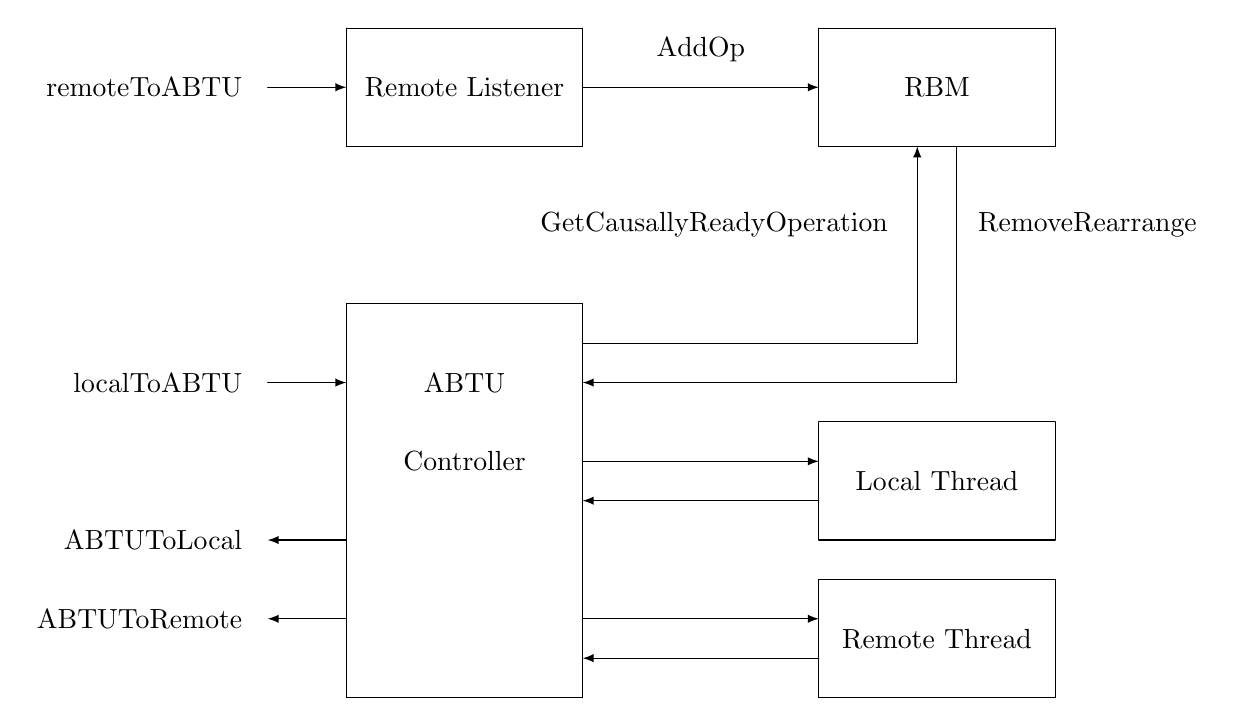
\begin{tikzpicture}[scale=1,cap=round, square/.style={regular polygon,regular polygon sides=4}]
\node at (-4.5, 1.75) {Remote Listener};
\draw (-6, 2.5) -- (-6, 1);
\draw (-6, 1) -- (-3, 1);
\draw (-3, 1) -- (-3, 2.5);
\draw (-3, 2.5) -- (-6, 2.5);

\node at (1.5, 1.75) {RBM};
\draw (0, 2.5) -- (0, 1);
\draw (0, 1) -- (3, 1);
\draw (3, 1) -- (3, 2.5);
\draw (3, 2.5) -- (0, 2.5);

\node at (-4.5, -2) {ABTU};
\node at (-4.5, -3) {Controller};
\draw (-6, -1) -- (-6, -6);
\draw (-6, -6) -- (-3, -6);
\draw (-3, -6) -- (-3, -1);
\draw (-3, -1) -- (-6, -1);

\node at (1.5, -3.25) {Local Thread};
\draw (0, -2.5) -- (0, -4);
\draw (0, -4) -- (3, -4);
\draw (3, -4) -- (3, -2.5);
\draw (3, -2.5) -- (0, -2.5);

\node at (1.5, -5.25) {Remote Thread};
\draw (0, -4.5) -- (0, -6);
\draw (0, -6) -- (3, -6);
\draw (3, -6) -- (3, -4.5);
\draw (3, -4.5) -- (0, -4.5);

%inputs
\draw (-7, 1.75) -- (-6, 1.75) [-latex];
\draw [-latex] (-7, -2) -- (-6, -2);
\draw [-latex] (-6, -4) --  (-7, -4);
\draw [-latex] (-6, -5) -- (-7, -5);

 \node at (-7.2, 1.75) [left] {remoteToABTU};
 \node at (-7.2, -2) [left] {localToABTU};
 \node at (-7.2, -4) [left] {ABTUToLocal};
 \node at (-7.2, -5) [left] {ABTUToRemote};
%inside
\draw (-3, 1.75) -- (0, 1.75) [-latex];
\node at (-1.5, 1.95) [above] {AddOp};

\draw (-3, -1.5) -- (1.25, -1.5);
\draw (1.25, -1.5) -- (1.25, 1) [-latex];
\node at (1, 0) [left] {GetCausallyReadyOperation};

\draw (1.75, 1) -- (1.75, -2);
\draw (1.75, -2) -- (-3, -2) [-latex];
\node at (1.9, 0) [right] {RemoveRearrange};

\draw [-latex] (-3, -3) -- (0, -3);
\draw [-latex] (0, -3.5) -- (-3, -3.5);

\draw [-latex] (-3, -5) -- (0, -5);
\draw [-latex] (0, -5.5) -- (-3, -5.5);
\end{tikzpicture}
\end{center}
\caption{The Big Picture. Own Illustration\label{fig:bigpic}}
\end{figure}

%---------------------------------------------------------------
\subsection{Communication with Peers}

The communication with other peers is done by using the go-libp2p library from \cite{libp2p}. This library implements advanced peer-to-peer communication features. The \textit{Run} function in figure~\ref{code:com} is inspired from the echo example in the go-libp2p repository from \cite{libp2p}.

The \textit{CommunicationService} struct contains a Host and two channels for sending and receiving operations. A peer is represented by the \textit{ABTUPeer} struct. As secured communication is not yet implemented, a random peer identity can be generated using the testutils.RandPeerID() function from the lib-p2p library.

In the \textit{Init} function, the peers are added to the host.Peerstore (4-8). In the Run function, messages from the mgmtToPeers channel are sent to all peers from the peerstore on the "epflDedisAbtu/Dispatch/0.0.1" protocol (20-28). On the other hand, incoming messages are put in the peersTomgmt channel in the streamHandler function (14-17).

With this simple design, the management can simply feed a channel to distribute messages and listen to a channel to receive messages.

\begin{figure}[!h]
\begin{center}
\begin{lstlisting}
func Init(myId SiteId, ABTUPeers map[SiteId]ABTUPeer)
	*CommunicationService {
	// ...
	for sId, ABTUPeer := range ABTUPeers {
		// ...
		host.Peerstore().
			AddAddr(peerId, multiAddress, pstore.PermanentAddrTTL)
	}
// ...
}
//...
func (comService *CommunicationService) Run()
	(chan<- []byte, <-chan []byte) {
	comService.host.SetStreamHandler(COMMUNICATION_PROTOCOL ,
							func(s net.Stream) {
		// ...
		comService.peersToMgmt <- incomingMsg
	})
	// ...
	go func () {
	for {
		outGoingMsg := <- comService.mgmtToPeers
		for _, peer := range comService.host.Peerstore().Peers() {
			// ...
			outGoingStream.Write(outGoingMsg)
		}
	}
	}()
}
// ...

\end{lstlisting}
\end{center}
\caption{Communication. Own Code.\label{code:com}}
\end{figure}

%---------------------------------------------------------------------------
\section{Results}

The following tests on the code base have been completed:
\begin{itemize}
	\item The receiving buffer manager is tested in the TestSimpleRequests function.
	\item Some unit tests have been written for the Timestamp struct, mostly for debugging.
\end{itemize}

The ABTU instance has been tested in three different ways:
\begin{enumerate}
	\item The TestOneABTUInstance from abtu1\_test.go simply feeds one ABTU instance with one local operation and one remote operation. The outgoing messages are simply printed out.
	\item The TestABTU2Instances connects two ABTU instances only with their respective channels. Two local operation and one undo are fed into the first instance which then communicates the resulting remote operations to the second instance. Messages are again printed in the console. The test function must answer to "remoteOperation" messages sent to the frontend to avoid a deadlock situation.
	\item The TestABTUWithCommunication1 from abtu1\_test.go and TestABTUWithCommunication2 from abtu2\_test.go work the same way as TestABTU2Instances but use the peer to peer communication. The ip addresses must be correctly set in the setupCommunicationService from abtu\_test.go.

This test can be done between two computers. As TestABTUWithCommunication2 is the receiver, it must be launched first, the thread then sleeps for 10 seconds to allow TestABTUWithCommunication1 to be launched. Messages are again printed out in the console.
\end{enumerate}

These tests show that the global design of the implementation is correct. However, they do not guarantee that the implementation of the algorithm is faultless. Further testing will have to be done in the future.

%-------------------------------------------------------------------------------------------------
\section{Limitations of the Project and Future Work}

A lot of effort has been put into the design of the implementation to allow for a good understanding and easy maintainability of the project. However, there is room for improvement in some areas.

For the moment, an ABTU instance can be started but not stopped correctly. The mechanism which stops the instance should recover the history buffer, time and receiving buffer. Furthermore, when a peer leaves the collaborative editing, other peers must be informed.

This leads to the second point: messages which are shared between peers only contain operations. There needs to be a more complex communication protocol in order to add features such as a peer leaving or joining a collaborative editing session.

The problem of peers joining is not easy to solve. Indeed, a joining site must first recover the state of the document, the corresponding time and history buffer from another site. Timestamps -  now basically implemented as slices of integers in a basic structure - also need to be extended for the joining of peers.

Another area where the implementation can be improved is error handling. For now, if an error occurs in the ABTU instance, the whole program simply fails with log.Fatal(). This has the repercussion of also crashing the management, thus making the frontend and the user completely clueless. An error should be recovered and error messages between the three parts of the software must be integrated in the communication protocol so that the management, frontend or user can be informed and react properly.

One of the main goals for the software this project is part of, is to make it as secure as possible. Adding security to the peer to peer communication would be a cornerstone for achieving this goal.

%------------------------------------------------------------------------------------------------
\section{Conclusion}

The first goal of the project is completed as the peer-to-peer communication between two sites has been implemented and is fully operational. The second goal is also completed as the implementation of an algorithm for peer-to-peer collaborative editing has been done. The third goal is partly achieved, as some basic tests have been done between two ABTU instances. The two last goals have not entirely been completed. The frontend, management and ABTU instance are almost ready for a linking. Nevertheless, there was not enough time left to properly join the three parts. For the the performance evaluation, a Go benchmarking file must be set up.

The next phase of the project would be to further test the implementation, evaluate its performance and terminate the linking with the management and frontend. More features could then be added to the software, such as stopping, managing errors, secure peer-to-peer communication and allow peers to join and leave the collaborative editing.

Algorithms for peer-to-peer collaborative editing is a complex but nonetheless interesting subject. The implementation of such an algorithm is challenging and requires a good understanding of the ABTU framework described in \cite{abtuu} and \cite{abtu}. Finally, the project of creating a complete software with an intuitive graphical interface is exciting. The work accomplished during this project will hopefully provide a solid base towards that aim!


\bibliography{biblio}{}
\bibliographystyle{alpha}
\pagebreak


%-------------------------------------------------------------------------------------------------------------------------------------------------------
\appendix
\section{Installation}
\label{appa}

The code of the project is available at \url{https://github.com/DamienAy/epflDedisABTU}. Go must be installed according to these instructions: \url{https://golang.org/doc/install}.
For the peer-to-peer communication, the go-libp2p library must be installed from \url{https://github.com/libp2p/go-libp2p}.

An ABTU instance can finally be instantiated and run with the code in figure~\ref{code:install}:

\begin{figure}[!h]
\begin{center}
\begin{lstlisting}
var siteId SiteId = 1
var numberOfSites int = 3
var initialSiteTimestamp Timestamp = NewTimestamp(numberOfSites)
var initialHistoryBuffer []Operation = make([]Operation, 0)
var initialRemoteBuffer []Operation = make([]Operation, 0)

// Instantiate
var abtu ABTUInstance =
	Init(siteId,
	      initialSiteTimestamp,
	      initialHistoryBuffer,
	     initialRemoteBuffer)

// Run
LocalToABTU, ABTUToLocal, RemoteToABTU , ABTUToRemote :=
	abtu.Run()
\end{lstlisting}
\end{center}
\caption{Instantiation of an ABTU Instance. Own Code.\label{code:install}}
\end{figure}

The communication service can be instantiated and run as shown in figure~\ref{code:installcom}.

\begin{figure}[!h]
\begin{center}
\begin{lstlisting}
var siteId SiteId = 1

peer1 := ABTUPeer{1,
	"QmVvtzcZgCkMnSFf2dnrBPXrWuNFWNM9J3MpZQCvWPuVZf",
	"127.0.0.1",
	"1234" }
peer2 := ABTUPeer{2,
	"QmT1VesmGjDy4LnGzqSAbkr7ntqh67cgedU2dhsMk7dVGL",
	"127.0.0.1",
	"1235" }

ABTUPeers := map[SiteId]ABTUPeer{1:peer1, 2:peer2}

// Instantiate
var comService CommunicationService = Init(siteId, ABTUPeers)

// Run
mgmtToPeers, peersToMgmt := comService.Run()

\end{lstlisting}
\end{center}
\caption{Instantiation of a Communication Service. Own Code.\label{code:installcom}}
\end{figure}

%-------------------------------------------------------------------------------------------------------------------------------------------------------
\section{Psoeudocode snaphots for local and remote thread}
The snapshots from figure~\ref{snap1},~\ref{snap2},~\ref{snap3} and ~\ref{snap4} provide from the \cite{abtuu} paper.

\begin{figure}[!h]
\begin{center}
\includegraphics[scale=0.5]{snapshots/localThread.jpg}
\end{center}
\caption{Local Thread. \cite{abtuu}.\label{snap1}}
\end{figure}

\begin{figure}[!h]
\begin{center}
\includegraphics[scale=0.5]{snapshots/integrateL.jpg}
\end{center}
\caption{IntegrateL. \cite{abtuu}.\label{snap2}}
\end{figure}

\begin{figure}[!h]
\begin{center}
\includegraphics[scale=0.5]{snapshots/remoteThread.jpg}
\end{center}
\caption{Remote Thread. \cite{abtuu}.\label{snap3}}
\end{figure}

\begin{figure}[!h]
\begin{center}
\includegraphics[scale=0.75]{snapshots/integrateR.jpg}
\end{center}
\caption{IntegrateR. \cite{abtuu}.\label{snap4}}
\end{figure}


\end{document}
